\documentclass{beamer}
\usepackage[T2A]{fontenc}
\usepackage[utf8]{inputenc}
\usepackage[russian]{babel}
\usepackage{color}
\usepackage{hyperref}
\usepackage{listings}
\usepackage{color}
\usepackage{graphicx}
\usetheme{default}

\setbeamertemplate{footline}[frame number]

\title{Определение демографических характеристик пользователей
сайта Last.fm на основе анализа их музыкальных интересов}
\author{\textbf{Семёнов~A.~C.,} \\ 
    магистрант кафедры КТ университета ИТМО, \\
    semkagtn@gmail.com}
\institute{СПИСОК 2016}
\date{\today}

\subject{Научно-исследовательская работа}

\AtBeginSection[]
{
  \begin{frame}<beamer>{Содержание}
    \tableofcontents[currentsection]
  \end{frame}
}

\AtBeginSubsection[]
{
  \begin{frame}<beamer>{Содержание}
    \tableofcontents[currentsection,currentsubsection]
  \end{frame}
}

\begin{document}

\begin{frame}
  \titlepage
\end{frame}

\begin{frame}{Содержание}
  \tableofcontents
\end{frame}

\section{Введение}

\begin{frame}{Интернет и его пользователи}
  \begin{itemize}
      \item {Огромное число пользователей}
          \begin{itemize}
              \item {Facebook~--- $968 \cdot 10^{6}$ уникальных посещений сайта в день}
              \item {Vkontakte~--- $75 \cdot 10^{6}$ уникальных посещений сайта в день}
              \item {Instagram~--- $400 \cdot 10^{6}$ уникальных посещений сайта в месяц}
          \end{itemize}
      \item {Информация о пользователях находится в открытом доступе}
          \begin{itemize}
              \item {Текст, который пишут пользователи}
              \item {Фотографии пользователей}
              \item {Интересы: фильмы, музыка, хобби}
              \item {Страна, город, геолокация}
              \item {Пол, возраст}
              \item {И т.д}
          \end{itemize}
  \end{itemize}
\end{frame}

\begin{frame}{Определение характеристик пользователей}
  \begin{itemize}
      \item {Информация о пользователях часто является не полной}
      \item {Задача: определить отсутствующие характеристики по имеющимся}
      \item {Определение пола и возраста по музыкальным предпочтениям пользоватлей}
  \end{itemize}
\end{frame}

\begin{frame}{Мотивация}
    \begin{itemize}
        \item {Пол и возраст~--- одни из ключевых характеристик,
            использующихся в рекомендательных системах}
        \item {Существует множество подходов к определению пола
            и возраста пользователей}
        \item {Информация о музыке пользователей используется не часто}
        \item {Метод определения пола и возраста по музыке
            может помочь улучшить существующие методы}
    \end{itemize}
\end{frame}

\section{Описание данных}

\begin{frame}{Источник данных~--- Last.fm}
    \begin{figure}
        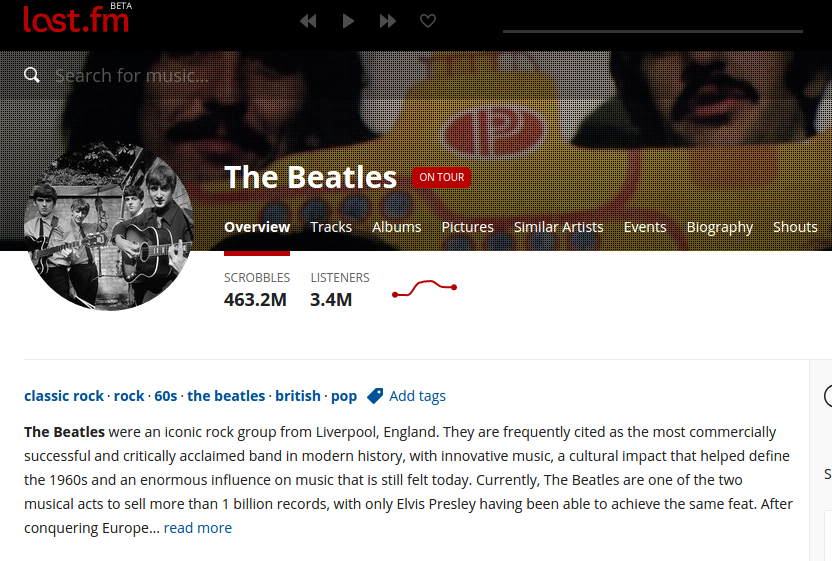
\includegraphics[width=\textwidth]{figures/lastfm.png}
    \end{figure}
\end{frame}

\begin{frame}{Набор данных}
    \begin{itemize}
        \item {Использовался набор данных из существующего 
              исследования~\footnote{Wu M. J.,
              Jang J. S. R., Lu C. H. Gender Identification
              and Age Estimation of Users Based on Music 
              Metadata // ISMIR. – 2014. – P.~555--560.}}
        \item {Всего $96807$ пользователей}
            \begin{itemize}
                \item {48404 пользователей в обучающей выборке}
                \item {48403 пользователей в контрольной выборке}
            \end{itemize}
        \item {Пользователь описан исполнителями из top-50 наиболее
            прослушиваемых им композиций}
        \item {У каждого пользователя указан пол и возраст}
        \item {66{,}2\% и 33{,}8\% мужчин и женщин соответственно}
        \item {Возраст пользователей смещён в сторону молодого поколения}
    \end{itemize}
\end{frame}

\begin{frame}{Иллюстрация задачи определения пола и возраста}
    \begin{figure}
        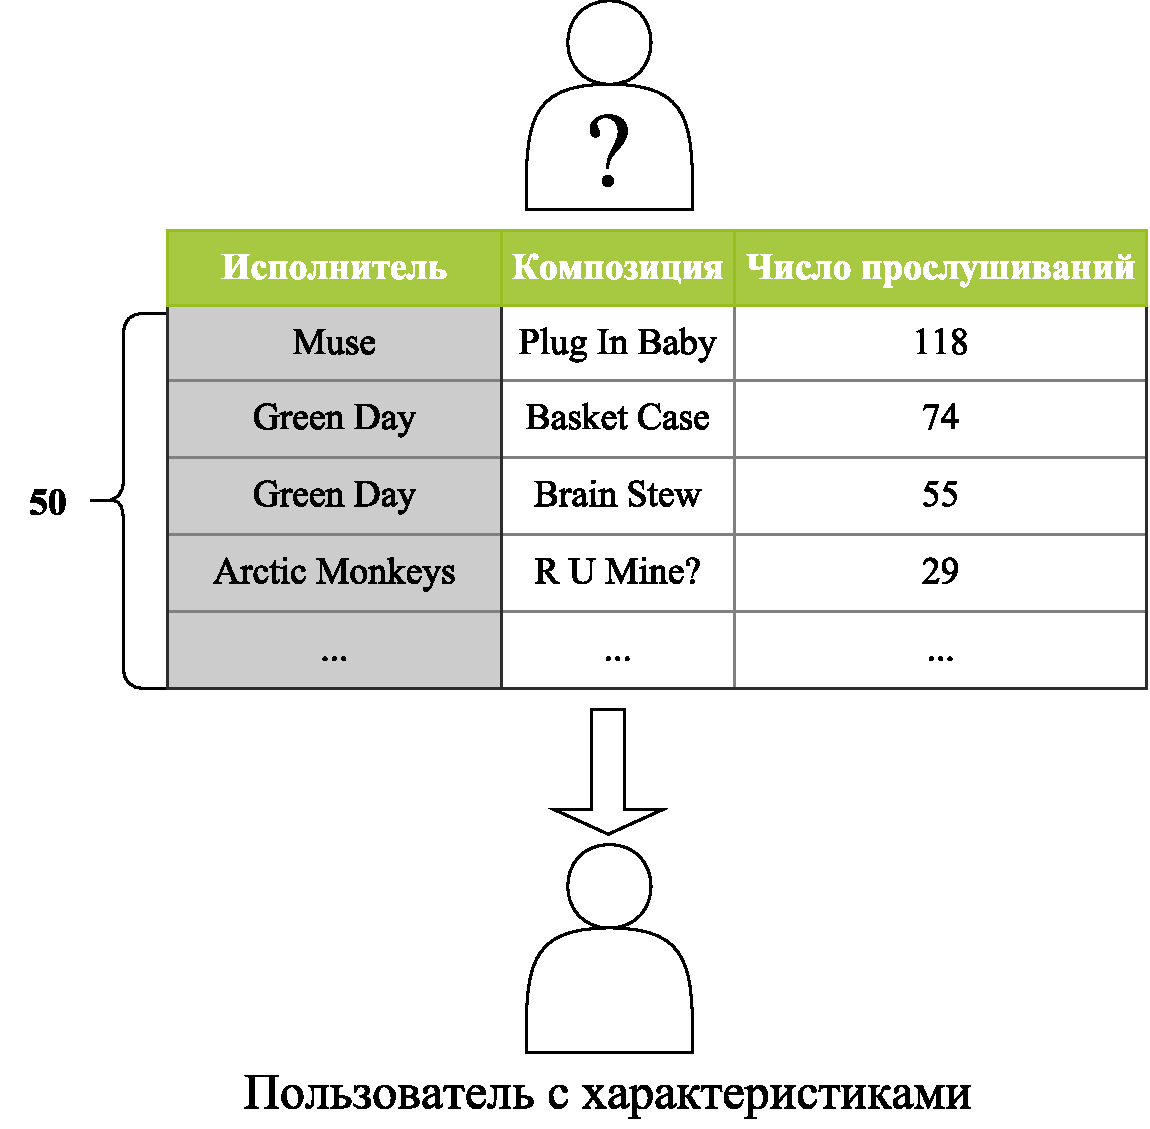
\includegraphics[scale=0.45]{figures/lastfm-top.pdf}
    \end{figure}
\end{frame}

\section{Преобразование данных в векторное пространство}

\subsection{Подход на основе матрицы термин--документ}

\begin{frame}{lol5}
  \begin{itemize}
      \item {}
  \end{itemize}
\end{frame}

\begin{frame}{lol6}
  \begin{itemize}
      \item {}
  \end{itemize}
\end{frame}

\subsection{Подход на основе модели Word2Vec}

\begin{frame}{lol7}
  \begin{itemize}
      \item {}
  \end{itemize}
\end{frame}

\begin{frame}{lol8}
  \begin{itemize}
      \item {}
  \end{itemize}
\end{frame}

\section{Этап обучения и результаты}

\begin{frame}{lol9}
  \begin{itemize}
      \item {}
  \end{itemize}
\end{frame}

\begin{frame}{lol0}
  \begin{itemize}
      \item {}
  \end{itemize}
\end{frame}

\begin{frame}[plain,c]
    \begin{center}
        \Huge Спасибо за внимание! Вопросы?
    \end{center}
\end{frame}

\end{document}
